\documentclass{siamart1116}

% basics
\usepackage[left=3cm,right=3cm,top=2.5cm,bottom=2.5cm]{geometry}
\usepackage[utf8x]{inputenc}
\usepackage[title,titletoc]{appendix}
\usepackage{afterpage}
\usepackage{enumitem}   
\setlist[enumerate]{topsep=3pt,itemsep=3pt,label=(\roman*)}

% maths
\usepackage{mathtools}
\usepackage{amsmath}
\usepackage{amssymb}
\newsiamremark{assumption}{Assumption}
\newsiamremark{remark}{Remark}
\newsiamremark{example}{Example}
\numberwithin{theorem}{section}

% tables
\usepackage{booktabs}

% plots
\usepackage{graphicx}
\usepackage{pgfplots}
\usepackage{tikz}
\usetikzlibrary{arrows,decorations.pathmorphing,backgrounds,positioning,fit,matrix}
\usepackage[labelfont=bf]{caption}
\usepackage{here}
\usepackage[font=normal]{subcaption}

% title and authors

\newcommand{\TheTitle}{Probabilistic geometric integration of Hamiltonian systems based on random time steps} 
\newcommand{\TheAuthors}{A. Abdulle, G. Garegnani}
\headers{Probabilistic symplectic integration of Hamiltonian systems}{\TheAuthors}
\title{{\TheTitle}}
\author{Assyr Abdulle\thanks{Institute of Mathematics, \'Ecole Polytechnique F\'ed\'erale de Lausanne (\email{assyr.abdulle@epfl.ch})}
		\and
		Giacomo Garegnani\thanks{Institute of Mathematics, \'Ecole Polytechnique F\'ed\'erale de Lausanne (\email{giacomo.garegnani@epfl.ch})}}

% my commands 
\DeclarePairedDelimiter{\ceil}{\left\lceil}{\right\rceil}
\DeclarePairedDelimiter{\floor}{\lfloor}{\rfloor}
\DeclarePairedDelimiter{\abs}{\lvert}{\rvert}
\DeclarePairedDelimiter{\norm}{\|}{\|}
\renewcommand{\phi}{\varphi}
\renewcommand{\theta}{\vartheta}
\renewcommand{\Pr}{\mathbb{P}}
\newcommand{\eqtext}[1]{\ensuremath{\stackrel{#1}{=}}}
\newcommand{\leqtext}[1]{\ensuremath{\stackrel{#1}{\leq}}}
\newcommand{\iid}{\ensuremath{\stackrel{\text{i.i.d.}}{\sim}}}
\newcommand{\totext}[1]{\ensuremath{\stackrel{#1}{\to}}}
\newcommand{\rightarrowtext}[1]{\ensuremath{\stackrel{#1}{\longrightarrow}}}
\newcommand{\leftrightarrowtext}[1]{\ensuremath{\stackrel{#1}{\longleftrightarrow}}}
\newcommand{\pdv}[2]{\ensuremath\partial_{#2}#1}
\newcommand{\N}{\mathbb{N}}
\newcommand{\R}{\mathbb{R}}
\newcommand{\C}{\mathbb{C}}
\newcommand{\OO}{\mathcal{O}}
\newcommand{\epl}{\varepsilon}
\newcommand{\diffL}{\mathcal{L}}
\newcommand{\prior}{\mathcal{Q}}
\newcommand{\defeq}{\coloneqq}
\newcommand{\eqdef}{\eqqcolon}
\newcommand{\Var}{\operatorname{Var}}
\newcommand{\E}{\operatorname{\mathbb{E}}}
\newcommand{\MSE}{\operatorname{MSE}}
\newcommand{\trace}{\operatorname{tr}}
\newcommand{\MH}{\mathrm{MH}}
\newcommand{\ttt}{\texttt}
\newcommand{\Hell}{d_{\mathrm{Hell}}}
\newcommand{\sksum}{{\textstyle\sum}}
\newcommand{\dd}{\mathrm{d}}
\definecolor{shade}{RGB}{100, 100, 100}
\definecolor{bordeaux}{RGB}{128, 0, 50}
\newcommand{\corr}[1]{{\color{red}#1}}

\ifpdf
\hypersetup{
	pdftitle={\TheTitle},
	pdfauthor={\TheAuthors}
}
\fi

\begin{document}
\maketitle

\begin{abstract} The long-time energy conservation of the random time stepping Runge-Kutta method (RTS-RK) introduced in [A. Abdulle and G. Garegnani, \textit{Random time step probabilistic methods for uncertainty quantification in chaotic and geometric numerical integration}, arXiv:1801.01340, 2018] is studied. Departing from classical backward error analysis tools, we show that the accumulation of errors due to random perturbations causes an energy drift which grows as the square root of time. Nonetheless, we are able to prove that the approximation in the mean sense of the Hamiltonian given by our probabilistic integrator has the same quality as an equivalent deterministic symplectic method over time spans of polynomial length. Numerical examples confirm our theoretical findings and show the effectiveness of the probabilistic approach in the frame of Bayesian inverse problems.
\end{abstract}

\section{Introduction}

Hamiltonian dynamics are used to model a variety of physical phenomena, such as celestial orbits or the dynamics of mechanical systems. All Hamiltonian system are endowed with the property of conserving an energy function which is specific to the considered dynamic. Mathematically, Hamiltonian systems can be modelled by an ordinary differential equations (ODE) which for a smooth energy function $Q\colon \R^{2d} \to \R$ and for an initial condition $y_0 \in \R^{2d}$ reads
\begin{equation}
y' = J^{-1}\nabla Q(y), \quad y(0) = y_0 \in \R^{2d},
\end{equation}
where the matrix $J$ is defined as
\begin{equation}
J = \begin{pmatrix} 0 & I \\ -I & 0 \end{pmatrix},
\end{equation}
and where $I$ is the $d$-dimensional identity matrix. The solution of the ODE above can be expressed in terms of the numerical flow $\phi_t \colon \R^{2d} \to \R^{2d}$ which maps the initial condition into the solution at a time $t > 0$, i.e., $y(t) = \phi_t(y_0)$. It is well known that the flow of Hamiltonian systems has the geometric property of conserving certain projected areas in the state space, or, in other words, it is symplectic. 

Symplectic Runge-Kutta methods are a class of numerical integrators which are particularly effective for Hamiltonian systems. In fact, the numerical flow of these methods preserves the geometric properties of the exact flow, which guarantees that the solution is accurate over long time spans. In particular, the energy of the system is nearly conserved along the trajectories of the numerical solution, where the accuracy depends on the chosen time step and on the method's order of convergence. Long-time conservation of energy and accuracy are relevant for many applications, e.g., in astronomy or molecular dynamics.

While the properties of energy conservation and long-time accuracy are fundamental for the integration of Hamiltonian systems, classical deterministic methods are associated only with a priori upper bounds for the numerical error, which can be insufficient for describing the method's accuracy in certain situations. In recent years, probabilistic numerical methods for integrating ODEs have been proposed  to provide a richer description of the approximation's quality \cite{AbG18, CGS16, KeH16, CCC16, SSH18}. The main idea underlying all these methods is to associate a probability measure to the punctual numerical solution given by classical methods, thus performing a consistent uncertainty quantification of the numerical error. This additional characterisation is particularly effective in the frame of problems of statistical inference, where applying classical schemes can lead to biased posterior concentrations and hence to inadequate solutions \cite{AbG18, COS17, CGS16}.

In our recent work \cite{AbG18} we introduced a probabilistic integrator of ODEs based on a random selection of time steps and explored the geometric properties of probabilistic methods. In particular, we focused on the numerical conservation of first integrals, showing theoretically and by means of numerical experiments that if a deterministic method conserves first integrals then randomisation of the time steps does not affect this property. Moreover, we showed that if the deterministic component has a symplectic flow, then the RTS-RK method has a symplectic flow. This does not imply directly that the energy conservation properties of symplectic integrators with fixed time steps are automatically inherited by randomised integrators as we cannot apply classical backward error analysis for constant time step symplectic methods. In fact, numerical experiments in \cite{AbG18} show that a symplectic RTS-RK method does not preserve the Hamiltonian. We recall that for deterministic symplectic integrators of order $q$ the Hamiltonian is preserved with accuracy $\OO(h^q)$ up to exponentially long time intervals.

Nevertheless, using backward error analysis we show in this paper that the Hamiltonian is preserved in the mean for a RTS-RK method built on a symplectic integrator. In particular, we are able to prove exploiting Brouwer's argument \cite{Bro37} that the mean deviation in energy is bounded and proportional to the square root of time. In particular, denoting by $q$ the order of the deterministic method, if the strenght of the noise introduced by the probabilistic method is well-balanced with the numerical error, we show that the mean energy drift is of order $\OO(h^q + t^{1/2}h^{2q})$. This result guarantees that for time intervals of size $t = \OO(h^{-2q})$ the probabilistic approximation preserves the mean energy with accuracy $\OO(h^q)$.

The paper is organised as follows. In section \ref{sec:BEA} we introduce the technique of backward error analysis for the quantification of errors, focusing on the classical results on energy conservation for Hamiltonian systems and symplectic methods. Then, in section \ref{sec:RTSBEA} we show the main theoretical result of this work, namely an energy conservation theorem for random time step integration. Finally, in section \ref{sec:NUMEXP} we present numerical experiments that illustrate our findings and we show an application of our method to Bayesian inverse problems.

\section{Background on backward error analysis}\label{sec:BEA} In this section we give a quick review on backward error analysis. For more details we refer to \cite{HLW06, LeR04, SaC94}. Let us consider a smooth function $f \colon \R^{2d} \to \R^{2d}$ and the ODE
\begin{equation}
	y' = f(y), \quad y(0) = y_0 \in \R^{2d}.
\end{equation}
We then consider a Runge-Kutta method identified by its numerical flow $\Psi_h \colon \R^{2d} \to \R^{2d}$, such that the numerical solution $y_n = \Psi_h^n(y_0)$ obtained applying $n$ times the flow $\Psi_h$ is an approximation of the solution $y(nh)$. The error introduced by time integration can be analysed via techniques of backward error analysis, whose key ingredient consists in finding a function $\tilde f\colon \R^{2d} \to \R^{2d}$ of the form $\tilde f(y) = f(y) + hf_2(y) + h^2 f_3(y) + \ldots$, such that the numerical solution is exact when applied to the system 
\begin{equation}
	y' = \tilde f(y), \quad y(0) = y_0.
\end{equation}
The functions $f_i, i = 2, 3, \ldots$ are built by matching the coefficients of equal powers of $h$ in the expression of $\tilde f$ and in the Taylor expansion of $\Psi_h$, which reads
\begin{equation}
	\Psi_h(y) = y + h f(y) + h^2 d_2(y) + h^3 d_3(y) + \ldots,  
\end{equation}
where the functions $d_i, i = 2, 3, \ldots$ depend on the derivatives of $f$ and on the coefficients of the Runge-Kutta method. Once an expression for $\tilde f$ is given, the numerical error is then analysed in terms of the difference between the modified and the original equation. A first result states that if the Runge-Kutta integrator has order $q$, then the lowest power of $h$ in the modified equation is again $q$, i.e.,
\begin{equation}
	\tilde f(y) = f(y) + h^q f_{q+1}(y) + h^{q+1} f_{q+2}(y) + \ldots,
\end{equation}
where the equality above is only formally true, as the series is not guaranteed to converge. In order to perform a rigorous backward error analysis it is hence necessary to choose a value $N > q$ and truncate the sum above after $N$ terms, thus getting
\begin{equation}
	\tilde f(y) = f(y) + h^q f_{q+1}(y) + h^{q+1} f_{q+2}(y) + \ldots + h^{N-1}f_N(y).
\end{equation}
We employ a slight abuse of notation, and in the following we always denote by $\tilde f$ the truncated modified function. 

We next focus on symplectic methods applied to Hamiltonian systems. Let us consider an analytic function $Q \colon \R^{2d} \to \R$ and the associated Hamiltonian system
\begin{equation}\label{eq:HamSystem}
y' = J^{-1}\nabla Q(y), \quad y(0) = y_0 \in \R^{2d}.
\end{equation}
Let us first recall the definition of a symplectic differentiable map.
\begin{definition}[Definition VI.2.2 in \cite{HLW06}] A differentiable map $g\colon U \to \R^{2d}$ (where $U\subset \R^{2d}$ is an open set) is called symplectic if the Jacobian matrix $g'$ is everywhere symplectic, i.e., if
\begin{equation}
	(g')^\top J g' = J.
\end{equation}	
\end{definition}
The exact flow map $\phi_t$ of an Hamiltonian system is symplectic. Moreover, we call a Runge-Kutta integrator symplectic if its flow map $\Psi_h$ is symplectic whenever it is applied to a smooth Hamiltonian system \cite{HLW06}. If a symplectic method is employed to integrate \eqref{eq:HamSystem}, it is known that the modified equation is still Hamiltonian, i.e., there exists a modified energy $\tilde Q \colon \R^{2d} \to \R$ defined as
\begin{equation}\label{eq:ModifiedHamiltonian}
\tilde Q(y) = Q(y) + h Q_2(y) + h^2 Q_3(y) + \ldots,
\end{equation}
such that $\tilde f = J^{-1}\nabla \tilde Q$. For the same reasons as above, it is more appropriate to consider the truncated Hamiltonian, which for an integrator of order $q$ reads
\begin{equation}\label{eq:ModifiedHamiltonianTrunc}
	\tilde Q(y) = Q(y) + h^q Q_{q+1}(y) + \ldots + h^{N-1} Q_N(y).
\end{equation}
As for the function $\tilde f$, let us remark that the notation $\tilde Q$ is used in the following to denote only the truncated Hamiltonian. Moreover, we denote by $\tilde \phi_{N, h}$ the exact flow of the dynamical system with Hamiltonian $\tilde Q$, highlighting the dependence on the truncation index $N$ and the time step $h$. In order to show results of energy conservation, it is necessary to introduce an assumption on the regularity of the dynamical system.

\begin{assumption}\label{as:RegHamiltonian} The function $f$ is analytic in a neighbourhood of the initial condition $y_0$ and there exist constants $M, R > 0$ such that $\norm{f(y)} \leq M$ for $\norm{y - y_0} \leq 2R$.
\end{assumption}

Under this assumption, it is possible to prove that the modified Hamiltonian $\tilde Q$ is Lipschitz continuous with a global constant independent of $h$ (see e.g. \cite{HLW06}, Section IX.7). Furthermore, a result of local error valid for any dynamical system and any Runge-Kutta method holds.

\begin{lemma}[see e.g. \cite{HLW06}, Section IX.7]\label{lem:LocalHamiltonianDet} Under assumption \ref{as:RegHamiltonian} and for $h$ sufficiently small, there exists $N = N(h)$ such that the numerical flow $\Psi_h$ and the exact flow of the truncated modified equation $\tilde \phi_{N, h}$ satisfy
	\begin{equation}
	\norm{\Psi_h(y_0) - \tilde \phi_{N, h}(y_0)} \leq C h e^{-\kappa / h},
	\end{equation}
	where $C$ and $\kappa$ are positive constants depending only on the method's coefficients and on the regularity of the function $f$.
\end{lemma}

In case of Hamiltonian systems and symplectic methods, the existence of a modified Hamiltonian guarantees that the error is small over long time spans. In particular, the following result holds.

\begin{theorem}[see e.g. \cite{HLW06}, Section IX.8] Under assumption \ref{as:RegHamiltonian} and for $h$ sufficiently small, the numerical solution $y_n$ given by a symplectic method of order $q$ applied to an Hamiltonian system satisfies
	\begin{align}
		\tilde Q(y_n) &= \tilde Q (y_0) + \OO(e^{-\kappa / 2h}), \\
		Q(y_n) &= Q(y_0) + \OO(h^q),
	\end{align}
	where the two results are valid for exponentially long times.
\end{theorem}

\section{Energy conservation with random time steps}\label{sec:RTSBEA} We now consider the random time stepping Runge-Kutta method (RTS-RK) introduced in \cite{AbG18}. Let us recall that this method is defined by the following recurrence relation
\begin{equation}\label{eq:RTSRK}
	Y_{n+1} = \Psi_{H_n}(Y_n), \quad Y_0 = y_0,
\end{equation}
where $\{H_i\}_{i\geq 0}$ is a sequence of independent and identically distributed (i.i.d.) positive random variables. The convergence and some geometric properties of this probabilistic numerical scheme have been studied in \cite{AbG18}. In particular, we report here the main assumption on the time steps which is needed for these properties to hold.
\begin{assumption}\label{as:AssumptionH} The i.i.d. random variables $H_k$ satisfy for all $k = 0, 1, \ldots$
	\begin{enumerate}
		\item\label{as:hStrong_Pos} $H_k > 0$ a.s.,
		\item\label{as:hStrong_E} there exists $h > 0$ such that $\E H_k = h$,
		\item\label{as:hStrong_Var} there exists $p \geq 1$ such that the scaled random variables $Z_k \defeq H_k - h$ satisfy
		\begin{equation}
		\E Z_k^2 = Ch^{2p},
		\end{equation}
		which is equivalent to $\E H_k^2 = h^2 + Ch^{2p}$.
	\end{enumerate}
\end{assumption}
We quickly summarise some results of \cite{AbG18}. Under Assumption \ref{as:AssumptionH} and for a deterministic integrator of order $q$, we have that the mean square convergence of the RTS-RK method is given by
\begin{equation}
	\big(\E\norm{Y_k - y(t_k)}^2\big)^{1/2}	\leq Ch^{\min\{q, p-1/2\}}, \quad k = 0, 1, \ldots, \quad t_k = kh,
\end{equation} 
while for any smooth function $\Phi \in \C^{\infty}(\R^d, \R)$ the weak convergence can be expressed as
\begin{equation}
	\abs{\E \Phi(Y_k) - \Phi(y(t_k))} \leq Ch^{\min\{q, 2p-1\}}, \quad k = 0, 1, \ldots, \quad t_k = kh.
\end{equation}
Let us finally recall the following result on the symplecticity of the flow of the RTS-RK method.

\begin{lemma}\label{lem:SympRTSRK} If the flow $\Psi_h$ of the deterministic integrator is symplectic, then the flow of the random time-stepping probabilistic method \eqref{eq:RTSRK} is symplectic.
\end{lemma}
This result implies that locally the random choice of the time steps does not destroy the geometric property of the underlying deterministic method. Nonetheless, this result is not sufficient to guarantee that energy is well conserved along the trajectories of the probabilistic method.

When integrating \eqref{eq:HamSystem} with the RTS-RK method, the perturbation introduced by the random choice of the time steps propagates in time following the system's dynamics. The accumulation of errors in the numerical solution of Hamiltonian systems has been treated in several works such as \cite{HMR08, Vil08b}. The main focus has been studying the impact of round-off errors on the conservation of energy when high-order symplectic method are employed. These works employ the so-called Brouwer's law \cite{Bro37}, which guarantees that the energy drift is proportional to the square root of time. In particular, let us denote as above by $y_n$ the $n$-th step of a symplectic integrator, which we assume for the moment to conserve exactly the Hamiltonian $Q$ (or equivalently any other quantity conserved by the ODE). Let us furthermore denote by $\bar y_n$ a perturbed numerical solution, which satisfies
\begin{equation}
	Q(y_n) - Q(\bar y_n) = Q(y_{n-1}) - Q(\bar y_{n-1}) + \xi_{n-1},
\end{equation}
where $\{\xi_i\}_{i\geq 0}$ is a sequence of zero-mean $i.i.d.$ random variables. Then there exists a constant $C > 0$ independent of $h$ such that
\begin{equation}\label{eq:Brower}
	\E\abs{Q(y_n) - Q(\bar y_n)} \leq C n^{1/2}.
\end{equation}
Let us remark that this argument holds for any quantity $L \colon \R^{2d} \to \R$ that is conserved by the flow of the differential equation. For general first integrals there is nonetheless no theoretical guarantee of good approximations over long time spans in the deterministic framework, hence we will focus in this work on Hamiltonian systems. We next prove our main result on the conservation of energy in Hamiltonian system for the RTS-RK method.

\begin{theorem}\label{thm:RTSHamiltonian} Under Assumptions \ref{as:RegHamiltonian} and \ref{as:AssumptionH} there exist constants $C_i > 0$, $i = 1, \ldots, 4$, such that the solution given by the RTS-RK method built on a symplectic deterministic method applied to a Hamiltonian system with Hamiltonian $Q$ satisfies
	\begin{align}
		\E \abs{\tilde Q(Y_n) - \tilde Q(y_0)} &\leq C_1 e^{-\kappa/2h}\big(1 + C_2 h^{2p-1}\big), \\
		\E \abs{Q(Y_n) - Q(y_0)} &\leq C_1 e^{-\kappa/2h}(1 + C_2 h^{2p-1}) + C_3 h^q + C_4 t^{1/2} h^{p+q-1/2}, \label{eq:ErrorHamiltonian}
	\end{align}
	where the first result is valid over exponentially long time intervals $nh \leq e^{\kappa / h}$.
\end{theorem}
\begin{proof} We exploit the conservation of $\tilde Q$ along the trajectories of its corresponding dynamical system, i.e., $\tilde Q (\tilde \phi_{N,z} (y)) = \tilde Q(y)$ for $y \in \R^d$ and $z > 0$ and employ a telescopic sum to obtain
\begin{equation}
\begin{aligned}
	\E \abs{\tilde Q(Y_n) - \tilde Q(y_0)} &\leq \sum_{j=1}^{n} \E\abs{(\tilde Q(Y_{j}) - \tilde Q(Y_{j-1})} \\
	&= \sum_{j=1}^{n} \E \abs{\tilde Q(Y_j) - \tilde Q(\tilde\phi_{N, H_{j-1}}(Y_{j-1}))} \\
	&= \sum_{j=1}^{n} \E\E\big(\abs{\tilde Q(Y_j) - \tilde Q (\tilde\phi_{N, H_{j-1}}(Y_{j-1}))} \mid H_{j-1}\big),
\end{aligned}
\end{equation}
where we applied the law of total expectation with respect to $H_{j-1}$ for the last equality. Then, as $\tilde Q$ is Lipschitz with constant independent of $h$ and under the assumptions on $\{H_i\}_{i\geq 0}$ and thanks to Lemma \ref{lem:LocalHamiltonianDet} we have
\begin{equation}
\begin{aligned}
\E \abs{\tilde Q(Y_n) - \tilde Q(y_0)} &\leq C \sum_{j=0}^{n-1} \E\big(H_{j}e^{-\kappa/H_j}\big)\\
&= C n \E\big(H_0e^{-\kappa/H_0}\big),
\end{aligned}
\end{equation}
where we exploited that the random time steps are \textit{i.i.d.} We can now consider the function $g(x) = xe^{-\kappa/x}$ and the bound
\begin{equation}
\begin{aligned}
	g(x) &\leq g(h) + g'(h) (x - h) + \frac{1}{2} \max_{x>0} g''(x) (x - h)^2 \\
	&\leq e^{-\kappa/h} \big(h + \frac{h + \kappa}{h}(x-h)\big) + \frac{27}{2\kappa}e^{-3} (x-h)^2, \quad x > 0,
\end{aligned}
\end{equation}
which is valid as $\max_{x>0} g''(x) = 27e^{-3}/\kappa$. Hence
\begin{equation}\label{eq:ErrorModifHamiltonian}
\begin{aligned}
\E \abs{\tilde Q(Y_n) - \tilde Q(y_0)} &\leq Cn \E\big( e^{-\kappa/h} \big(h + \frac{h + \kappa}{h}(H_0-h)\big) + \frac{27}{\kappa}e^{-3} (H_0-h)^2 \big) \\
&= Cnhe^{-\kappa/h}(1 + \frac{27}{\kappa}e^{-3} h^{2p-1}) \\
&\leq Ce^{-\kappa/2h}(1 + \frac{27}{\kappa}e^{-3} h^{2p-1}),
\end{aligned}
\end{equation}
where the equality is given by the assumptions on $H_0$. Hence, the first result is proved with $C_1 = C$ and $C_2 = 27e^{-3}/\kappa$. We now consider the original Hamiltonian $Q(y)$. We have by the triangular inequality
\begin{equation}
	\E\abs{Q(Y_n) - Q(y_0)} \leq \E\abs{Q(Y_n) - \tilde Q(Y_n)} + \E\abs{\tilde Q(Y_n) - \tilde Q(y_0)} + \abs{\tilde Q(y_0) - Q(y_0)}.
\end{equation}
The second term is bounded thanks to \eqref{eq:ErrorModifHamiltonian}, and the third is of order $\OO(h^q)$ from \eqref{eq:ModifiedHamiltonianTrunc}. For the first term, let us denote by $R(y) = Q(y) - \tilde Q(y)$ and by $y_n$ the numerical solution obtained with fixed time steps and the same symplectic integrator as the RTS-RK method. We apply the triangular inequality again and obtain
\begin{equation}
	\E\abs{R(Y_n)} \leq \E\abs{R(Y_n) - R(y_n)} + \abs{R(y_n)}.
\end{equation}
For the second term, we have $\abs{R(y)} \leq Mh^q$ for some constant $M > 0$. For the first term, we now expand $R(Y_n)$ with the Taylor expansion of both the numerical flow $\Psi_t$ and of the function $R$ to obtain
\begin{equation}
	R(Y_n) = R(Y_{n-1}) + R'(Y_{n-1})H_{n-1}\sum_{i=1}^{s}b_i J^{-1}\nabla Q(Y_{n-1}) + \OO(H_{n-1}^2),
\end{equation} 
where $s$ is the number of stages of the Runge-Kutta method and the scalar coefficients $\{b_i\}_{i=1}^s$ are its weights. Let us remark that under Assumption \ref{as:RegHamiltonian}, there exist a constant $M$ such taht $R'(y) \leq M h^q$ and $J^{-1}\nabla Q(y) \leq M$. Moreover, we can write a similar expansion for the solution $y_n$ obtained with fixed time step $h$ and get
\begin{equation}
	R(Y_n) - R(y_n) = R(Y_{n-1}) - R(y_{n-1}) + h^q \xi_{n-1},
\end{equation}
where $\xi_{n-1} \propto (H_{n-1} - h)$ is a zero-mean random variable with standard deviation proportional to $h^p$. We can then conclude by \eqref{eq:Brower} that
\begin{equation}
	\E\abs{R(Y_n) - R(y_n)} \leq C n^{1/2} h^{p+q},
\end{equation}
where $C$ is a positive constant independent of $h$ and $n$, which concludes the proof.
\end{proof}

\begin{remark} The two results implied by Theorem \ref{thm:RTSHamiltonian} are consistent with the theory of deterministic symplectic integrators. In fact, in the limit $p \to \infty$, we have
	\begin{align}
		\E \abs{\tilde Q(Y_n) - \tilde Q(y_0)} &= \OO(e^{-\kappa/h}), \\
		\E \abs{Q(Y_n) - Q(y_0)} &= \OO(h^q),
	\end{align}
	and the expectation $\E Q(Y_n) \to Q(y_n)$, where $y_n$ is the numerical solution given by the deterministic method.
\end{remark}
\begin{remark} If we choose $p = q + 1/2$ and disregarding the first term on the right hand side of expression \eqref{eq:ErrorHamiltonian} as it decreases exponentially with $h$, we have
\begin{equation}\label{eq:OptimalNoiseScale}
	\E\abs{Q(Y_n) - Q(y_0)} \leq C_3 h^q + C_4t^{1/2}h^{2q},
\end{equation} 
which guarantees that $\E\abs{Q(Y_n) - Q(y_0)} = \OO(h^q)$ for time intervals of length $t = \OO(h^{-2q})$. Let us remark that this is the same accuracy that would be obtained employing a deterministic symplectic method. Nonetheless, the RTS-RK approximation is valid over polynomial time spans instead of exponential time spans as in the deterministic case.
\end{remark}

\section{Numerical experiments}\label{sec:NUMEXP}
In this section we illustrate by two numerical experiments the finding of Theorem \ref{thm:RTSHamiltonian}. Moreover, we consider the inverse problem of retrieving the initial condition of an Hamiltonian system from a single observation of its state at some time $t > 0$, showing how a probabilistic approach can be employed in this framework.

\subsection{Convergence}\label{sec:NumConv}
\begin{figure}[t!]
	\centering
	\includegraphics[]{ConvMean}
	\caption{Convergence of the mean error on the Hamiltonian for the Hénon-Heiles problem. The dashed lines represent theoretical estimates given by expression \eqref{eq:ErrorHamiltonian}, while the solid lines represent the experimental results. The mean was computed averaging 100 realisations of the numerical solution.}
	\label{fig:Mean}	
\end{figure}

Let us consider the Hénon-Heiles system, which is given by the Hamiltonian $Q \colon \R^4 \to \R$ defined by
\begin{equation}\label{eq:HamHH}
	Q(v, w) = \frac{1}{2}\norm{v}^2 + \frac{1}{2}\norm{w}^2 + w_1^2w_2 - \frac{1}{3}w_2^3,
\end{equation}
where $y = (v, w)^\top \in \R^4$. We consider an initial condition such that $Q(y_0) = 0.13$ and integrate the equation employing the RTS-RK method using the two stage Gauss collocation method, which is symplectic and of order $q = 4$, and the noise scale $p = \{2, 4\}$. The time steps are drawn from a uniform distribution $\mathcal{U}(h-h^p, h-h^p)$, so that Assumption \ref{as:AssumptionH} is satisfied. We vary the mean time step $h_i = 0.2 \cdot 2^{-i}$ for $i = 0, \ldots, 7$ and consider the final time $T = 10^4$ for both values of $p$. We then compute the value of $Q$ at final time and compare it with $Q(y_0)$ to check numerically the validity of Theorem \ref{thm:RTSHamiltonian}. Results are shown in Figure \ref{fig:Mean}, where the dashed and dotted lines are given by the left hand side of \eqref{eq:ErrorHamiltonian} disregarding the first term, i.e., $C_3h^q + C_4t^{1/2}h^{p+q-1/2}$, with $C_3 = 3\cdot 10^{-2}$, $C_4 = 2\cdot 10^{-4}$. We observe that for small values of $h$ the slope of the error decreases as the asymptotic regime is reached.

\subsection{Error growth} Let us consider the pendulum problem, which is given by the Hamiltonian $Q \colon \R^2 \to \R$ defined by

\begin{figure}[t]
	\centering
	\includegraphics[]{MeanTime2}
	\caption{Time evolution of the mean error for the pendulum problem and different values of the time step $h$. The black lines represent the theoretical estimate given by the left hand side of equation \eqref{eq:OptimalNoiseScale}, while the colored lines represent the experimental results. The mean was computed averaging 20 realisations of the numerical solution.}
	\label{fig:MeanTime}	
\end{figure}
\begin{equation}
	Q(v, w) = \frac{v^2}{2} - \cos w,
\end{equation}
where $y = (v, w)^\top \in \R^2$. We consider the initial condition $(v_0, w_0) = (1.5, -\pi)$ and integrate the equation employing RTS-RK based on the implicit midpoint method ($q = 2$) and $p = q + 1/2 = 2.5$, which is the optimal scaling of the noise. We wish to study the validity of \eqref{eq:OptimalNoiseScale}, i.e., show that the error on the mean Hamiltonian grows as the square root of time after when the term of order $\OO(t^{1/2}h^{2q})$ becomes dominant with respect to the term of order $\OO(h^q)$. Hence, we vary the mean time step $h \in \{0.2, 0.1, 0.05, 0.025\}$, integrate the dynamical system up to the final time $T = 10^6$ and study the time evolution of the numerical error on the Hamiltonian $Q$. Results are shown in Figure \ref{fig:MeanTime}, where it is possible to notice that the error is growing with a rate $1/2$ in time after a stationary phase, where the term in $h^q$ in \eqref{eq:OptimalNoiseScale} is dominating the term in $t^{1/2}h^{2q}$ due to the lower power of $h$. The oscillations of the error which are shown in Figure \ref{fig:StdTime} are due to the term of order $h^q$ and are present even when integrating the pendulum system deterministically with a symplectic scheme. Moreover, we show in Figure \ref{fig:StdTime} the time evolution up to final time $T = 10^4$ of the mean and of the standard deviation of the energy, which is as well proportional to $t^{1/2}h^{2q}$, with the final distribution of the samples which ressembles a Gaussian distribution.

\begin{figure}[t]
	\centering
	\includegraphics[]{StdTime}
	\caption{Samples from the numerical solution and time evolution of the standard deviation. Solid gray lines represent the energy over all the 200 considered trajectories, the solid black line is the mean energy, the dashed line is the standard deviation and the dotted line is the theoretical estimation of the energy deviation.}
	\label{fig:StdTime}	
\end{figure}

\subsection{Bayesian inverse problem} Let us consider a Hamiltonian system with energy $Q(v,w)$ and exact flow $\phi_t$. We are interested in recovering the true value of the initial condition $y_0$ through a single observations $y_{\mathrm{obs}}$ of the solution $(v, w)$ at time $t = t_{\mathrm{obs}}$. The initial condition is chosen as in Section \ref{sec:NumConv} to be such that $Q(y_0) = 0.13$. We assume that the observation is corrupted by an additive source of noise that we describe as a Gaussian random variable $\epl \sim \mathcal{N}(0, \sigma_\epl^2 I)$, i.e., $y_{\mathrm{obs}} = \phi_{t_{\mathrm{obs}}}(y_0) + \epl$. We interpret this inverse problem in the Bayesian sense and thus specify a Gaussian prior $\pi_{\mathrm{prior}} = \mathcal{N}(0, I)$ on the initial condition, so that we have by Bayes' theorem that the true posterior distribution reads
\begin{equation}\label{eq:PosteriorExact}
\begin{aligned}
	\pi(\tilde y_0 \mid y_{\mathrm{obs}}) &\propto \pi_{\mathrm{prior}}(\tilde y_0) \pi(y_{\mathrm{obs}} \mid \tilde y_0)\\
	&\propto \exp\Big(-\frac{\tilde y_0^\top \tilde y_0}{2} -\frac{(\phi_{t_{\mathrm{obs}}}(\tilde y_0) - y_{\mathrm{obs}})^\top(\phi_{t_{\mathrm{obs}}}(\tilde y_0) - y_{\mathrm{obs}})}{2\sigma_\epl^2}\Big),
\end{aligned}
\end{equation}
where $\pi(y_{\mathrm{obs}} \mid \tilde y_0)$ is the likelihood of the observation with respect to an initial condition $\tilde y_0$. In order to compute the posterior distribution, it is necessary to introduce a numerical approximation of the equation's flow. If we denote by $\Psi_h^{n_{\mathrm{obs}}}(\tilde y_0)$ with $n_{\mathrm{obs}} = t_{\mathrm{obs}} / h$ a deterministic approximation obtained applying $n$ times the numerical flow $\Psi_h$ to the initial condition $\tilde y_0$, the approximation of the posterior reads
\begin{equation}\label{eq:PosteriorDet}
	\pi^h_{\mathrm{det}}(\tilde y_0 \mid y_{\mathrm{obs}}) \propto \exp\Big(-\frac{\tilde y_0^\top \tilde y_0}{2} -\frac{(\Psi_h^{n_{\mathrm{obs}}}(\tilde y_0) - y_{\mathrm{obs}})^\top(\Psi_h^{n_{\mathrm{obs}}}(\tilde y_0) - y_{\mathrm{obs}})}{2\sigma_\epl^2}\Big).
\end{equation}
Let us now denote by $\mathbf{H} = (H_0, H_1, \ldots, H_{n_\mathrm{obs}})^\top$ the set of random time steps employed for numerical integration with the RTS-RK method. We can compute the posterior distribution marginalising over the random variable $\mathbf{H}$, thus obtaining
\begin{equation}\label{eq:PosteriorProb}
	\pi^h_{\mathrm{prob}}(\tilde y_0 \mid y_{\mathrm{obs}}) \propto \exp\Big(-\frac{\tilde y_0^\top \tilde y_0}{2}\Big) \E^{\mathbf{H}} \exp\Big(-\frac{(\Psi_\mathbf{H}(\tilde y_0) - y_{\mathrm{obs}})^\top(\Psi_\mathbf{H}(\tilde y_0) - y_{\mathrm{obs}})}{2\sigma_\epl^2}\Big),
\end{equation}
where $\Psi_\mathbf H(\tilde y_0) = (\Psi_{H_{n_{\mathrm{obs}}-1}} \circ \Psi_{H_{n_{\mathrm{obs}}-2}} \circ \ldots \circ \Psi_{H_0})(\tilde y_0)$ is the probabilistic numerical approximation of $\phi_{t_{\mathrm{obs}}}(\tilde y_0)$ given by the RTS-RK method and $\E^\mathbf{H}$ is the expectation with respect to the random variable $\mathbf{H}$. Let us remark that the convergence with respect to $h \to 0$ of the distributions defined in \eqref{eq:PosteriorDet} and \eqref{eq:PosteriorProb} to the true posterior distribution \eqref{eq:PosteriorExact} is guaranteed under some regularity assumptions over the exact forward model, i.e., the exact flow $\phi_{t_{\mathrm{obs}}}$ (see e.g., \cite{Stu10} Section 4 for the deterministic approximation and \cite{LST17} for a general framework with random posterior distributions).
Let us consider the Hénon-Heiles equation, given by the Hamiltonian \eqref{eq:HamHH}. A classical second-order ($q = 2$) symplectic method is the Störmer-Verlet scheme \cite{Sto07, Ver67, HLW06}, for which one step is defined in the general case as
\begin{equation}
\begin{aligned}
	v_{n+1/2} &= v_n - \frac{h}{2} \nabla_w Q(v_n, w_n), \\
	w_{n+1} &= w_n + \frac{h}{2} \big(\nabla_v Q(v_{n+1/2}, w_n) + \nabla_v Q(v_{n+1/2}, w_{n+1})\big),\\
	v_{n+1} &= v_{n+1/2} - \frac{h}{2} \nabla_w Q(v_{n+1/2}, w_{n+1}).
\end{aligned}
\end{equation}
As the Hamiltonian $Q$ given by \eqref{eq:HamHH} is separable, i.e., $Q(v, w) = Q_1(v) + Q_2(w)$, where $Q_1, Q_2 \colon \R^2 \to \R$, the Störmer-Verlet scheme simplifies to
\begin{equation}
\begin{aligned}
	v_{n+1/2} &= v_n - \frac{h}{2} \nabla_w Q_2(w_n), \\
	w_{n+1} &= w_n + h \nabla_v Q_1(v_{n+1/2}),\\
	v_{n+1} &= v_{n+1/2} - \frac{h}{2} \nabla_w Q_2(w_{n+1}).
\end{aligned}
\end{equation}
Hence, the evaluation of the flow of the RTS-RK method consists only of three evaluations of the derivatives of $Q$, instead of the solution of a nonlinear system. 

In order to sample from the posterior distributions $\pi^h_{\mathrm{det}}$ and $\pi^h_{\mathrm{prob}}$ we employ the Metropolis-Hastings (MH) and the pseudo-marginal Metropolis-Hastings (PMMH) algorithms. Given an initial guess $\tilde y_0^{(0)}$, these algorithms fix a proposal distribution $q \colon \R^d\times \R^d \to \R$ which is measurable in its first argument and a probability density function in its second argument and produce $M$ samples from the posterior distribution by the following procedure
\begin{enumerate}
	\item Compute $\pi(\tilde y_0^{(0)} \mid y_{\mathrm{obs}})$ and set $i = 0$;
	\item Propose a new value $\tilde y_0^{\dagger}$ sampling from $q(\tilde y_0^{(i)}, \cdot)$;
	\item With probability 
	\begin{equation}
		\alpha(\tilde y_0^{(i)}, \tilde y_0^{\dagger}) = \min\Big\{ \frac{\pi(\tilde y_0^\dagger \mid y_{\mathrm{obs}}) q(\tilde y_0^{\dagger}, \tilde y_0^{(i)})}
		{\pi(\tilde y_0^{(i)} \mid y_{\mathrm{obs}}) q(\tilde y_0^{(i)}, \tilde y_0^{\dagger})} , 1\Big\}
	\end{equation}
	set $\tilde y_0^{(i+1)} = \tilde y_0^{\dagger}$, otherwise set $\tilde y_0^{(i+1)} = \tilde y_0^{(i)}$;
	\item if $i < M$, set $i \leftarrow i + 1$ and return to step (ii).
\end{enumerate}
Further details on how to employ these algorithms for RTS-RK methods can be found in \cite{AbG18}. We then consider $t_{\mathrm{obs}} = 10$, the standard deviation of the observational noise $\sigma_\epl = 5 \cdot 10^{-4}$ and the time step $h = \{0.2, 0.1, 0.05, 0.025\}$ for numerical integration. The approximated marginal posterior distributions of $ y_0 = (v_{0,1}, v_{0, 2}, w_{0, 1}, w_{0, 2})$ are shown in Figure \ref{fig:Bayes}. In particular, we have
\begin{itemize}[label = -]
	\item Figure \ref{fig:BayesA}: $\Psi_h$ is approximated via Heun's method \cite{Heu00} ($q = 2$), which is given by the numerical flow 
	\begin{equation*}
		\Psi_h(y_n) = y_n + \frac{h}{2}\Big(f(y_n) + f\big(y_n + hf(y_n)\big)\Big),
	\end{equation*}
	\item Figure \ref{fig:BayesB}: $\Psi_h$ is approximated via the Störmer-Verlet method,
	\item Figure \ref{fig:BayesC}: $\Psi_h$ is approximated via the RTS-RK Störmer-Verlet method with the natural choice $p = q+1/2 = 5/2$.
\end{itemize}
We can observe that the posterior distributions given by Heun's method are concentrated away from the true value of the initial condition for the larger values of the time step. In fact, Heun's method is not symplectic, and a deviation on the energy $Q$ is produced when integrating in time the dynamical system. Hence, initial conditions with a different energy level with respect to the observation are endowed with a high value of likelihood and the resulting posterior distribution is concentrated far from the true value. This behaviour is corrected using the Störmer-Verlet method thanks to its symplecticity. However, we remark in Figure \ref{fig:BayesB} that the posterior distribution for $h = 0.2$ is still concentrated on a biased value of the initial condition, without any indication of this bias given by the posterior's variance. Applying the RTS-RK method together with PMMH instead gives nested posterior distributions whose variance quantifies the uncertainty of the numerical solver. This favourable behaviour is possible thanks to the numerical error quantification of probabilistic methods, which has been already shown in \cite{AbG18, CGS16, COS17}, together with the good energy conservation properties of the RTS-RK method when a symplectic integrator is used as its deterministic component as proved in Theorem \ref{thm:RTSHamiltonian}.

\begin{figure}
\begin{subfigure}{\textwidth}
	\centering
	\includegraphics[]{BayesHeun}
	\includegraphics[]{BayesHeun2}
	\caption{$\pi^h_{\mathrm{det}}(y_0\mid y_{\mathrm{obs}})$, Heun}
	\label{fig:BayesA}
\end{subfigure}	
\begin{subfigure}{\textwidth}
	\centering
	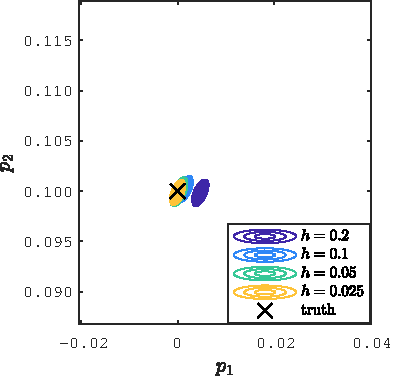
\includegraphics[]{BayesDet}
	\includegraphics[]{BayesDet2}
	\caption{$\pi^h_{\mathrm{det}}(y_0\mid y_{\mathrm{obs}})$, Störmer-Verlet}
	\label{fig:BayesB}
\end{subfigure}
\begin{subfigure}{\textwidth}
	\centering
	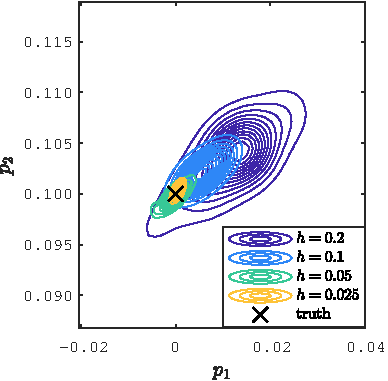
\includegraphics[]{BayesProb}
	\includegraphics[]{BayesProb2}
	\caption{$\pi^h_{\mathrm{prob}}(y_0\mid y_{\mathrm{obs}})$, RTS-RK Störmer-Verlet}
	\label{fig:BayesC}
\end{subfigure}
\caption{Deterministic posterior distribution for Heun's and Störmer-Verlet schemes and probabilistic posterior distribution for the RTS-RK Störmer-Verlet scheme for various values of the time step $h$. The cross corresponds to the true value of the initial condition that is employed to generate the observation.}
\label{fig:Bayes}
\end{figure}

\def\cprime{$'$}
\begin{thebibliography}{10}
	
	\bibitem{AbG18}
	{\sc A.~Abdulle and G.~Garegnani}, {\em Random time step probabilistic methods
		for uncertainty quantification in chaotic and geometric numerical
		integration}, arXiv preprint arXiv:1801.01340,  (2018).
	
	\bibitem{Bro37}
	{\sc D.~Brouwer}, {\em On the accumulation of errors in numerical integration},
	Astronomical Journal, 46 (1937), pp.~149--153.
	
	\bibitem{CCC16}
	{\sc O.~A. Chkrebtii, D.~A. Campbell, B.~Calderhead, and M.~A. Girolami}, {\em
		Bayesian solution uncertainty quantification for differential equations},
	Bayesian Anal., 11 (2016), pp.~1239--1267.
	
	\bibitem{COS17}
	{\sc J.~Cockayne, C.~Oates, T.~Sullivan, and M.~Girolami}, {\em Probabilistic
		numerical methods for {PDE}-constrained {B}ayesian inverse problems}, AIP
	Conference Proceedings, 1853 (2017), p.~060001.
	
	\bibitem{CGS16}
	{\sc P.~R. Conrad, M.~Girolami, S.~S{\"a}rkk{\"a}, A.~Stuart, and
		K.~Zygalakis}, {\em Statistical analysis of differential equations:
		introducing probability measures on numerical solutions}, Stat. Comput.,
	(2016).
	
	\bibitem{HLW06}
	{\sc E.~Hairer, C.~Lubich, and G.~Wanner}, {\em Geometric Numerical
		Integration. Structure-Preserving Algorithms for Ordinary Differential
		Equations}, Springer Series in Computational Mathematics 31, Springer-Verlag,
	Berlin, second~ed., 2006.
	
	\bibitem{HMR08}
	{\sc E.~Hairer, R.~McLachlan, and A.~Razakarivony}, {\em Achieving {B}rouwer's
		law with implicit {R}unge-{K}utta methods}, BIT, 48 (2008), pp.~231--243.
	
	\bibitem{Heu00}
	{\sc K.~Heun}, {\em Neue {M}ethode zur approximativen {I}ntegration der
		dif\-feren\-tial\-gleichungen einer unabh\"angigen ver\"anderlichen},
	Zeitschr.\ f\"ur Math.\ u.\ Phys., 45 (1900), pp.~23--38.
	
	\bibitem{KeH16}
	{\sc H.~Kersting and P.~Hennig}, {\em Active uncertainty calibration in
		{B}ayesian {ODE} solvers}, in Proceedings of the 32nd Conference on
	Uncertainty in Artificial Intelligence (UAI 2016), {AUAI} Press, 2016,
	pp.~309--318.
	
	\bibitem{LeR04}
	{\sc B.~Leimkuhler and S.~Reich}, {\em Simulating {H}amiltonian {D}ynamics},
	Cambridge Monographs on Applied and Computational Mathematics 14, Cambridge
	University Press, Cambridge, 2004.
	
	\bibitem{LST17}
	{\sc H.~C. Lie, T.~Sullivan, and A.~Teckentrup}, {\em Random forward models and
		log-likelihoods in bayesian inverse problems}, arXiv preprint
	arXiv:1712.05717,  (2017).
	
	\bibitem{SaC94}
	{\sc J.~M. Sanz-Serna and M.~P. Calvo}, {\em Numerical {H}amiltonian
		{P}roblems}, Chapman \& Hall, London, 1994.
	
	\bibitem{SSH18}
	{\sc M.~Schober, S.~S{\"a}rkk{\"a}, and P.~Hennig}, {\em A probabilistic model
		for the numerical solution of initial value problems}, Stat. Comput.,
	(2018).
	
	\bibitem{Sto07}
	{\sc C.~St\"ormer}, {\em Sur les trajectoires des corpuscules \'electris\'es},
	Arch.\ sci.\ phys.\ nat. Gen\`eve, 24 (1907), pp.~5--18, 113--158, 221--247.
	
	\bibitem{Stu10}
	{\sc A.~M. Stuart}, {\em Inverse problems: A {B}ayesian perspective}, Acta
	Numer., 19 (2010), pp.~451--559.
	
	\bibitem{Ver67}
	{\sc L.~Verlet}, {\em Computer ``experiments'' on classical fluids. i.
		thermodynamical properties of {L}ennard-{J}ones molecules}, Physical Review,
	159 (1967), pp.~98--103.
	
	\bibitem{Vil08b}
	{\sc G.~Vilmart}, {\em Reducing round-off errors in rigid body dynamics}, J.
	Comput. Phys., 227 (2008), pp.~7083--7088.
	
\end{thebibliography}

\end{document}
